\documentclass[12pt,a3paper, landscape]{article}
\usepackage[utf8]{inputenc} 
\usepackage[ngerman]{babel}
\usepackage[T1]{fontenc}
\usepackage{amsmath}
\usepackage{amsfonts}
\usepackage{amssymb}
\usepackage{graphicx}
\usepackage[left=2cm,right=2cm,top=2cm,bottom=2cm]{geometry}
\usepackage{physics}
\usepackage{float}
\usepackage{multirow}
\setlength{\parindent}{0pt}
\usepackage{enumitem}
\usepackage{xcolor}
\usepackage{cancel} 

\newcommand{\h}[2]{\color{#1} #2 \color{black} }

\newcommand{\equalInM}[1]{\h{blue}{#1}} % umfasst mehr; inkl. Vorzeichen gleich über Sym-Anti und Anti-Sym und über die versch. Tableaus dieser Kategorie
\newcommand{\equalInTableau}[1]{\h{magenta}{#1}} % Vorzeichen vertauscht zw. den versch. Tableaus, aber Vorzeichen gleich bzgl. Anti-Sym zu Sym-Anti-Tausch
\newcommand{\equalAntiSym}[1]{\h{brown}{#1}} % zwar nicht in allen Tableaus einer M Sorte, aber gleich (inkl. Vorzeichen) bzgl. der Anti-Sym und der Sym-Anti Rechnung



\usepackage{soul}   % Für das Hervorheben von Text
\usepackage{booktabs}
\usepackage{hhline}
\usepackage{array}
\usepackage{adjustbox}


\begin{document}
\footnotesize

\begin{adjustbox}{width=\textwidth,totalheight=\textheight,keepaspectratio}


\begin{tabular}{|p{0.5cm}p{1.5cm}p{1cm}
!{\vline width 2pt}p{1cm}p{1cm}p{1cm}p{1cm}p{1cm}!{\vline width 1.25pt}
p{1cm}p{1cm}p{1cm}|p{1cm}p{1cm}p{1cm}|p{1cm}p{1cm}p{1cm}
!{\vline width 1.25pt}p{2cm}p{2cm}|}
\hline 
& && \multicolumn{5}{c!{\vline width 1.25pt}}{$\left[ 4\right]$ } & \multicolumn{9}{c!{\vline width 1.25pt}}{ $\left[ 3\; 1 \right]$}  & \multicolumn{2}{c|}{$\left[ 2^2\right]$}\\
 & && \multicolumn{5}{c!{\vline width 1.25pt}}{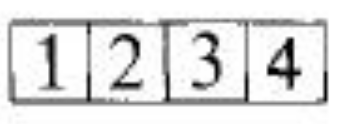
\includegraphics[scale=0.1]{build/young-4.png}} & 
  \multicolumn{3}{c|}{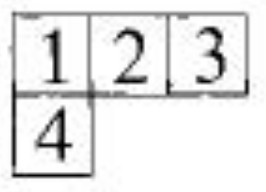
\includegraphics[scale=0.1]{young-31-123.png} } &  
  \multicolumn{3}{c|}{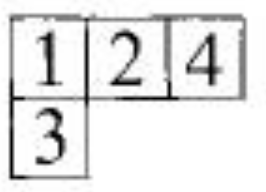
\includegraphics[scale=0.1]{young-31-124.png}} &  
  \multicolumn{3}{c!{\vline width 1.25pt}}{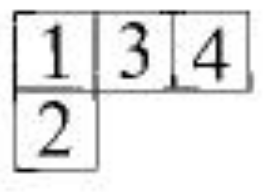
\includegraphics[scale=0.1]{young-31-134.png} }&  
 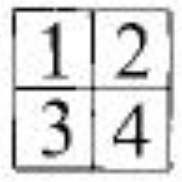
\includegraphics[scale=0.1]{young-2hoch2-12.png} & 
 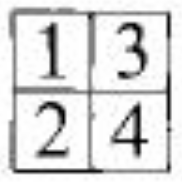
\includegraphics[scale=0.1]{young-2hoch2-13.png}  \\  
 &&&
 $\ket{2\;2}$ &  $\ket{2\;1}$ &  $\ket{2\;0}$  &  $\ket{2\;-1}$  &  $\ket{2\;-2}$  
 & $\ket{1\;1}$  & $\ket{1\;0}$  & $\ket{1\;-1}$ 
 & $\ket{1\;1}$  & $\ket{1\;0}$  & $\ket{1\;-1}$ 
 & $\ket{1\;1}$  & $\ket{1\;0}$  & $\ket{1\;-1}$  
 &  $\ket{0\;0}$ &  $\ket{0\;0}$
 \\ \specialrule{0.2em}{0em}{0em}
 $\left[ 4\right]$ & 
 \multirow{5}{*}{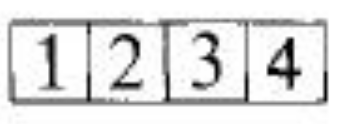
\includegraphics[scale=0.1]{build/young-4.png} }& 
 $\ket{2\;2}$ &1&0&0&0&0        & 0&0&0&0&0&0&0&0&0&   0&0\\
 & & $\ket{2\;1}$ &0&1&0&0&0    & 0&0&0&0&0&0&0&0&0&   0&0\\
 &&  $\ket{2\;0}$  & 0&0&1&0&0  & 0&0&0&0&0&0&0&0&0&   0&0\\
 && $\ket{2\;-1}$  & 0&0&0&1&0  & 0&0&0&0&0&0&0&0&0&   0&0\\
 && $\ket{2\;-2}$  & 0&0&0&0&1  & 0&0&0&0&0&0&0&0&0&   0&0
 \\ \specialrule{0.125em}{0em}{0em}
\multirow{3}{*}{$\left[ 3\; 1 \right]$} 
			&  \multirow{3}{*}{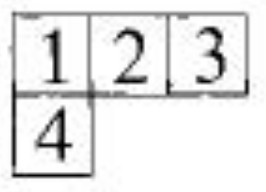
\includegraphics[scale=0.1]{young-31-123.png} }
			& $\ket{1\;1}$ &0&0&0&0&0&  1&0&0&      1/2&0&0&   1/2&0&0&  0&0\\
			&& $\ket{1\;0}$ &0&0&0&0&0&  0&1&0&     0&1/2&0&   0&1/2&0&  0&0\\
			&& $\ket{1\;-1}$ &0&0&0&0&0&  0&0&1&    0&0&1/2&   0&0&1/2&  0&0\\ \cline{2-19}
			&   \multirow{3}{*}{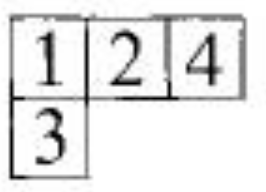
\includegraphics[scale=0.1]{young-31-124.png} }
			& $\ket{1\;1}$  &0&0&0&0&0& 1/2&0&0&   1&0&0&    1/2&0&0&    0&0\\
			&& $\ket{1\;0}$ &0&0&0&0&0&  0&1/2&0   &0&1&0&    0&1/2&0&   0&0\\
			&& $\ket{1\;-1}$ &0&0&0&0&0& 0&0&1/2   &0&0&1 &    0&0&1/2&  0&0\\ \cline{2-19}
			&   \multirow{3}{*}{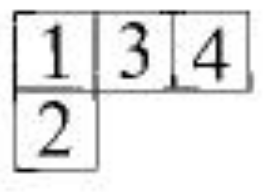
\includegraphics[scale=0.1]{young-31-134.png} }
			& $\ket{1\;1}$   &0&0&0&0&0&   1/2&0&0&    1/2&0&0&    1&0&0&  0&0  \\
			&& $\ket{1\;0}$  &0&0&0&0&0&   0&1/2&0&    0&1/2&0&    0&1&0&  0&0\\
			&& $\ket{1\;-1}$ &0&0&0&0&0&   0&0&1/2&   0&0&1/2&     0&0&1&  0&0\\
			 \specialrule{0.125em}{0em}{0em}
\multirow{2}{*}{$\left[ 2^2\right]$} 
			& 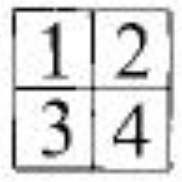
\includegraphics[scale=0.1]{young-2hoch2-12.png} 
			& $\ket{0\;0}$ &0&0&0&0&0&  0&0&0&0&0&0&0&0&0&   1&1/2\\
			& 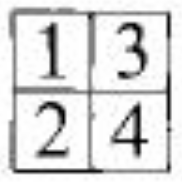
\includegraphics[scale=0.1]{young-2hoch2-13.png} 
			& $\ket{0\;0}$ &0&0&0&0&0&	0&0&0&0&0&0&0&0&0&   1/2&1\\
			\hline 
\end{tabular}\\




\end{adjustbox}




\end{document}